\documentclass[pdflatex,sn-basic,Numbered]{sn-jnl}

\usepackage{graphicx}
\usepackage{multirow}
\usepackage{amsmath,amssymb,amsfonts}
\usepackage{booktabs}
\usepackage{xcolor}
\usepackage{url}
\usepackage{subcaption}

\graphicspath{{images/}}
% Authoritative Scientific Metrics Macros Generated Automatically
% Do NOT manually edit this file. Regenerate via python_analysis/generate_paper_artifacts.py

% --- Dataset & Preprocessing ---
\newcommand{\DatasetTotalRecords}{253,680}
\newcommand{\ClassZeroCount}{218,334}
\newcommand{\ClassZeroPct}{86.07\%}
\newcommand{\ClassOneCount}{35,346}
\newcommand{\ClassOnePct}{13.93\%}
\newcommand{\ExactDuplicateSurplus}{24,206}
\newcommand{\ExactDuplicateSurplusPct}{9.54\%}
\newcommand{\ExactDuplicateInGroups}{35,575}
\newcommand{\ExactDuplicateInGroupsPct}{14.02\%}
\newcommand{\ExactDuplicateDistinctGroups}{11,369}
\newcommand{\UniquePredictorProfiles}{227,908}
\newcommand{\ProfileSurplus}{25,772}
\newcommand{\ProfileSurplusPct}{10.16\%}
\newcommand{\ProfileInGroups}{38,000}
\newcommand{\ProfileInGroupsPct}{14.98\%}
\newcommand{\ConflictingProfiles}{1,566}
\newcommand{\ConflictingObservations}{5,218}
\newcommand{\ConflictingObsPct}{2.06\%}

% --- Split & Evaluation Integrity ---
\newcommand{\DevSampleSize}{202,944}
\newcommand{\HoldoutSampleSize}{50,736}
\newcommand{\HoldoutProfileOverlapCount}{6,836}
\newcommand{\HoldoutProfileOverlapPct}{13.47\%}
\newcommand{\HoldoutExactRowOverlapCount}{6,375}
\newcommand{\HoldoutExactRowOverlapPct}{12.56\%}

% --- Machine Learning Model Selection & CV ---
\newcommand{\BestModelName}{XGBoost}
\newcommand{\SelectedThreshold}{0.13}
\newcommand{\XGBMeanCvPrAuc}{0.4359}
\newcommand{\XGBStdCvPrAuc}{0.0077}
\newcommand{\XGBMeanCvRocAuc}{0.8305}
\newcommand{\XGBStdCvRocAuc}{0.0021}
\newcommand{\RFMeanCvPrAuc}{0.4301}
\newcommand{\LRMeanCvPrAuc}{0.4163}
\newcommand{\DTMeanCvPrAuc}{0.4015}

% --- Primary Holdout Test Evaluation ---
\newcommand{\PrimaryHoldoutPrAuc}{0.4238}
\newcommand{\PrimaryHoldoutPrAucCiLower}{0.4135}
\newcommand{\PrimaryHoldoutPrAucCiUpper}{0.4347}
\newcommand{\PrimaryHoldoutRocAuc}{0.8272}
\newcommand{\PrimaryHoldoutRocAucCiLower}{0.8223}
\newcommand{\PrimaryHoldoutRocAucCiUpper}{0.8322}
\newcommand{\PrimaryHoldoutRecall}{80.99\%}
\newcommand{\PrimaryHoldoutRecallCiLower}{80.04\%}
\newcommand{\PrimaryHoldoutRecallCiUpper}{81.94\%}
\newcommand{\PrimaryHoldoutPrecision}{29.91\%}
\newcommand{\PrimaryHoldoutPrecisionCiLower}{29.53\%}
\newcommand{\PrimaryHoldoutPrecisionCiUpper}{30.28\%}
\newcommand{\PrimaryHoldoutSpecificity}{69.28\%}
\newcommand{\PrimaryHoldoutFOne}{0.4369}
\newcommand{\PrimaryHoldoutFalseNegativeReduction}{77.22\%}
\newcommand{\PrimaryHoldoutBrier}{0.0974}
\newcommand{\PrimaryHoldoutBrierCiLower}{0.0964}
\newcommand{\PrimaryHoldoutBrierCiUpper}{0.0983}
\newcommand{\PrimaryHoldoutCalibSlope}{0.9589}
\newcommand{\PrimaryHoldoutCalibSlopeCiLower}{0.9342}
\newcommand{\PrimaryHoldoutCalibSlopeCiUpper}{0.9854}
\newcommand{\PrimaryHoldoutCalibIntercept}{-0.0515}
\newcommand{\PrimaryHoldoutCalibInterceptCiLower}{-0.0861}
\newcommand{\PrimaryHoldoutCalibInterceptCiUpper}{-0.0148}

% --- SHAP & Statistical Consensus (RQ3) ---
\newcommand{\ShapConsensusTopFiveJaccard}{1.0000}
\newcommand{\ShapConsensusTopTenJaccard}{1.0000}
\newcommand{\ShapConsensusTopFifteenJaccard}{0.7647}
\newcommand{\ShapConsensusSpearmanRho}{0.9338}
\newcommand{\ShapConsensusSpearmanPValue}{6.38e-10}
\newcommand{\ShapMinusDfTopTenOverlap}{10}
\newcommand{\ShapMinusDfTopTenJaccard}{1.0000}
\newcommand{\ShapMinusDfSpearmanRho}{0.9338}
\newcommand{\ShapDivDfTopTenOverlap}{9}
\newcommand{\ShapDivDfTopTenJaccard}{0.8182}
\newcommand{\ShapDivDfSpearmanRho}{0.8818}

% --- Profile-Grouped Sensitivity Evaluation (RQ4) ---
\newcommand{\GroupedHoldoutPrAuc}{0.4372}
\newcommand{\GroupedHoldoutPrAucCiLower}{0.4256}
\newcommand{\GroupedHoldoutPrAucCiUpper}{0.4478}
\newcommand{\GroupedHoldoutRocAuc}{0.8310}
\newcommand{\GroupedHoldoutRocAucCiLower}{0.8262}
\newcommand{\GroupedHoldoutRocAucCiUpper}{0.8353}
\newcommand{\GroupedHoldoutRecall}{81.54\%}
\newcommand{\GroupedHoldoutRecallCiLower}{80.65\%}
\newcommand{\GroupedHoldoutRecallCiUpper}{82.43\%}
\newcommand{\GroupedHoldoutPrecision}{29.93\%}
\newcommand{\GroupedHoldoutPrecisionCiLower}{29.55\%}
\newcommand{\GroupedHoldoutPrecisionCiUpper}{30.30\%}
\newcommand{\GroupedHoldoutSpecificity}{69.10\%}
\newcommand{\GroupedHoldoutBrier}{0.0964}
\newcommand{\GroupedHoldoutCalibSlope}{0.9878}
\newcommand{\GroupedHoldoutCalibIntercept}{-0.0158}


\begin{document}

\title[Predicting Diabetes Risk Using CDC Health Indicators]{Predicting Diabetes Risk Using CDC Health Indicators: An Interpretable Machine Learning, Evidence Alignment, and Evaluation Integrity Framework}

\author*[1]{\fnm{Phan Tuan} \sur{Dat}}\email{ptundatwork@gmail.com}
\author[1]{\fnm{Lam Huynh} \sur{Khang}}\email{khanglhse200666@fpt.edu.vn}
\author[1]{\fnm{Nguyen Trong} \sur{Nhan}}\email{nhan@gmail.com}
\affil*[1]{\orgdiv{Artificial Intelligence}, \orgname{FPT University}, \orgaddress{\city{Ho Chi Minh City}, \country{Vietnam}}}

\abstract{
Early identification of diabetes risk from self-reported health survey data is vital for population health surveillance and community screening. Using the 2015 Behavioral Risk Factor Surveillance System (BRFSS) dataset ($N = 253,680$; 21 predictors; 13.93\% positive prevalence of prediabetes or diabetes), this study develops an interpretable machine learning pipeline paired with non-parametric statistical hypothesis testing, probability calibration, and an explicit evaluation-integrity audit. We evaluated four supervised classification algorithms under a conventional 80/20 stratified development/holdout split ($n_{\text{dev}} = 202,944$; $n_{\text{holdout}} = 50,736$) using 5-fold cross-validation. XGBoost achieved the highest observed mean cross-validated Precision-Recall Area Under the Curve (PR-AUC = $0.4359 \pm 0.0077$) and Receiver Operating Characteristic Area Under the Curve (ROC-AUC = $0.8305 \pm 0.0021$) among prespecified configurations, followed by Random Forest (PR-AUC 0.4301), Logistic Regression (PR-AUC 0.4163), and Decision Tree (PR-AUC 0.4015). To align predictions with population screening objectives, decision thresholds were selected on development out-of-fold probabilities, establishing an operational cutoff of 0.13 to target $\ge 80\%$ recall. Evaluated once on the untouched independent holdout set, the selected model achieved ROC-AUC of 0.8272 (95\% CI: [0.8223, 0.8322]), PR-AUC of 0.4238 (95\% CI: [0.4135, 0.4347]), recall of 80.99\% (95\% CI: [80.04\%, 81.94\%]), precision of 29.91\% (95\% CI: [29.53\%, 30.28\%]), and specificity of 69.28\%, decreasing the count of false negatives by 77.22\% (from 5,900 to 1,344) compared with the default 0.50 threshold. Holdout calibration assessment yielded a Brier score of 0.0974, a calibration slope of 0.9589 (95\% CI: [0.9342, 0.9854]), and an intercept of $-0.0515$ (95\% CI: [$-0.0861$, $-0.0148$]), reflecting a modest systematic calibration deviation while preserving close alignment across deciles. SHAP TreeExplainer attributions exhibited strong rank concordance with multivariable statistical likelihood contributions (Spearman $\rho_s = 0.9338$, $p = 6.38 \times 10^{-10}$; Top-5 and Top-10 Jaccard similarity = 1.0000). Furthermore, a profile-grouped sensitivity analysis eliminating cross-partition sharing of identical predictor profiles yielded broadly similar discrimination, screening performance, and calibration estimates (holdout PR-AUC 0.4372, ROC-AUC 0.8310, recall 81.54\%, Brier score 0.0964, calibration slope 0.9876), providing additional evidence that the study's primary internal conclusions are robust to the evaluated partitioning strategy.
}

\keywords{Diabetes Risk Prediction, CDC BRFSS, Explainable AI, SHAP, Probability Calibration, Screening Threshold, Evaluation Integrity, Sensitivity Analysis}

\maketitle

\section{Introduction}\label{sec:intro}

Diabetes mellitus is a major chronic disease that poses severe challenges to healthcare systems worldwide, substantially elevating the risk of cardiovascular events, stroke, neuropathy, nephropathy, and premature mortality \cite{ada2024standards}. Early identification of individuals at elevated risk can enable timely behavioral interventions, clinical diagnostics, and lifestyle counseling. Large-scale public health surveillance systems, such as the Behavioral Risk Factor Surveillance System (BRFSS) conducted by the Centers for Disease Control and Prevention (CDC), collect valuable population-level health, lifestyle, and behavioral data across hundreds of thousands of annual participants \cite{cdc2015brfss}. 

With the maturation of data science, numerous studies have explored supervised machine learning algorithms to predict diabetes status using BRFSS indicators \cite{uci2023brfss,ullah2022detecting,mani2012type}. However, critical methodological gaps persist in the literature:
\begin{enumerate}
    \item \textbf{Metric Misalignment Under Class Imbalance:} The positive prevalence of prediabetes or diabetes in public BRFSS samples is approximately 13.93\%. Despite this substantial imbalance, many studies report overall accuracy or ROC-AUC without reporting Precision-Recall curves (PR-AUC), which can mask poor predictive utility in the minority class \cite{saito2015precision}.
    \item \textbf{Neglect of Operational Decision Thresholds:} Off-the-shelf classifiers typically apply a default 0.50 probability cutoff. In low-prevalence screening contexts, this default threshold generates excessive false negatives, missing upwards of 80\% of individuals with diabetes \cite{steyerberg2010assessing}.
    \item \textbf{Uncalibrated Risk Estimates:} Clinical and public health decision-makers require accurate absolute risk estimates. Most machine learning pipelines omit formal probability calibration diagnostics such as Brier scores and Cox calibration curves \cite{vancalster2016calibration}.
    \item \textbf{Lack of Explanatory Grounding:} Machine learning explanations (e.g., SHAP attributions) are frequently presented as isolated feature rankings without verifying whether they concord with classical non-parametric and multivariable epidemiological effect sizes \cite{lundberg2020local}.
    \item \textbf{Evaluation Integrity and Repeated Profiles:} BRFSS variables are predominantly discrete and ordinal. In large samples, multiple respondents inevitably share identical combinations of predictor variables. When conventional random train-test splitting is applied, identical predictor profiles cross evaluation partitions. Existing studies rarely audit this phenomenon or perform sensitivity analyses to evaluate whether cross-partition profile sharing affects evaluation reliability \cite{kaufman2012leakage,kapoor2023leakage}.
\end{enumerate}

To address these limitations, this paper establishes a reproducible, end-to-end framework combining statistical inference, screening-oriented machine learning evaluation, probability calibration, SHAP evidence alignment, and a rigorous evaluation-integrity audit. Specifically, we investigate four core research questions:
\begin{itemize}
    \item \textbf{RQ1 (Statistical Associations):} Which demographic, behavioral, and clinical indicators exhibit statistically robust sample-level associations with reported diabetes status in the CDC BRFSS 2015 dataset?
    \item \textbf{RQ2 (Screening Predictive Modeling):} Which supervised classifier and development-selected decision threshold maximize screening sensitivity while maintaining acceptable precision on an independent internal holdout sample?
    \item \textbf{RQ3 (Exploratory Internal Evidence Alignment):} To what extent do model-level SHAP attributions concord with classical non-parametric and multivariable statistical effect sizes on the same underlying observational data?
    \item \textbf{RQ4 (Evaluation Robustness and Sensitivity):} To what extent are the study's discrimination and calibration findings stable when identical predictor profiles are prevented from crossing evaluation partitions?
\end{itemize}

\section{Related Work}\label{sec:related}

\subsection{Machine Learning for Diabetes Prediction}
Extensive research has investigated machine learning models for diabetes prediction using electronic health records (EHR) and survey data \cite{mani2012type,ullah2022detecting}. While EHR datasets contain rich biomarkers (e.g., fasting plasma glucose, HbA1c), public health surveillance datasets like the CDC BRFSS rely exclusively on self-reported survey responses. Studies using the BRFSS 2015 indicators have reported ROC-AUC values between 0.80 and 0.83 using ensemble methods such as Random Forest and XGBoost \cite{chen2016xgboost,breiman2001random}. However, many existing studies evaluate models using unadjusted classification thresholds or report metrics without confidence intervals, obscuring uncertainty in practical deployment.

\subsection{Threshold Optimization and Probability Calibration}
In community screening, the cost of a false negative (failing to identify an individual with diabetes) far exceeds the cost of a false positive (recommending a follow-up diagnostic blood test) \cite{steyerberg2010assessing}. Saito and Rehmsmeier \cite{saito2015precision} demonstrated that the PR-AUC is more informative than ROC-AUC when evaluating imbalanced datasets, as ROC curves can present an overly optimistic picture when the true negative class is large. Furthermore, modern tree ensembles frequently output uncalibrated probabilities that cannot be interpreted as posterior risks without calibration assessment \cite{vancalster2016calibration,cox1958two}.

\subsection{Explainable Artificial Intelligence (XAI)}
SHAP (SHapley Additive exPlanations), grounded in cooperative game theory, provides a mathematically unified measure of feature attribution \cite{lundberg2017unified,lundberg2020local}. While SHAP is widely applied in healthcare analytics, model-based explanations can capture non-linear or conditional interactions that do not align with marginal statistical associations. Systematically cross-referencing SHAP rankings with classical epidemiological effect sizes provides an essential validation layer against spurious algorithmic artifacts.

\subsection{Data Integrity, Evaluation Robustness, and Repeated Profiles in Survey Data}
While classical data leakage involves direct information transfer from test to training partitions \cite{kaufman2012leakage,kapoor2023leakage}, discretized survey datasets present a distinct evaluation-integrity concern through repeated predictor profiles. If identical profiles appear in both training and test sets, flexible models could theoretically memorize recurring patterns rather than generalizing to novel respondent profiles. Evaluating survey-based models therefore benefits from quantifying cross-partition predictor-profile sharing and conducting sensitivity analyses that enforce zero-overlap partitions.

\section{Data and Preprocessing}\label{sec:data}

\subsection{Dataset Description}
This study uses the cleaned 2015 BRFSS Diabetes Health Indicators dataset made publicly accessible via the UCI Machine Learning Repository \cite{uci2023brfss}. The dataset comprises $N = 253,680$ survey respondents and 21 predictor variables spanning sociodemographic characteristics, health behaviors, clinical history, and healthcare utilization. The binary target variable, \texttt{Diabetes\_binary}, categorizes respondents into Class 0 (no reported diabetes; $n = 218,334$, 86.07\%) and Class 1 (reported prediabetes or diabetes; $n = 35,346$, 13.93\%). No missing values are present in the dataset.

\subsection{Data Integrity Audit: Exact Duplicates versus Predictor Profiles}
Prior literature has frequently noted the presence of duplicate observations in this dataset, often casually reporting ``24,206 duplicate rows'' without distinguishing full-row duplicates from repeated predictor profiles. To resolve this ambiguity, we conducted a formal data integrity audit:
\begin{itemize}
    \item \textbf{Exact Full-Row Duplication:} When all 22 columns (21 predictors plus \texttt{Diabetes\_binary}) are considered, there are 24,206 surplus exact duplicate rows, involving 35,575 total observations clustered across 11,369 distinct response patterns.
    \item \textbf{Predictor-Profile Repetition:} When profiles are defined strictly across the 21 predictor variables (excluding the target), there are 227,908 unique predictor profiles. Among these, 12,228 profiles appear multiple times, representing 25,772 surplus observations and 38,000 total records.
    \item \textbf{Conflicting-Label Profiles:} Crucially, 1,566 predictor profiles contain conflicting target labels (i.e., some respondents sharing the profile report diabetes while others do not). These conflicting profiles encompass 5,218 observations (2.06\% of the total dataset).
\end{itemize}

All repeated observations were deliberately retained in the primary analyzed dataset because identical discrete response profiles may legitimately occur among different respondents, and respondent identity cannot be determined from the released analytic dataset. In a large survey sample with discrete and ordinal variables (e.g., binary indicators, 13 age categories, 8 income brackets), multiple independent individuals can legitimately report identical health attributes; assuming they represent duplicate individuals would be scientifically unfounded and would distort empirical population sample distributions. The summary of the dataset and integrity audit is presented in Table \ref{tab:data_overview}.

\begin{table}[htbp]
\centering
\caption{Dataset Summary and Integrity Audit Overview}
\label{tab:data_overview}
\begin{tabular}{lc}
\toprule
\textbf{Metric / Parameter} & \textbf{Value} \\
\midrule
Total Analyzed Observations ($N$) & 253,680 \\
Number of Predictor Variables & 21 \\
Target Variable & \texttt{Diabetes\_binary} \\
Class 0: No reported diabetes & 218,334 (86.07\%) \\
Class 1: Prediabetes or diabetes & 35,346 (13.93\%) \\
Missing Values & 0 (0.00\%) \\
\midrule
\multicolumn{2}{l}{\textit{Data Integrity Audit: Duplication and Profiles}} \\
Surplus Exact Duplicate Rows (22 variables) & 24,206 (9.54\%) \\
Observations in Exact Duplicate Clusters & 35,575 (14.02\%) \\
Distinct Exact Duplicate Groups & 11,369 \\
Unique Predictor Profiles (21 predictors only) & 227,908 \\
Surplus Repeated Predictor Profiles & 25,772 (10.16\%) \\
Observations in Repeated Predictor Profiles & 38,000 (14.98\%) \\
Distinct Multi-Observation Predictor Profiles & 12,228 \\
Predictor Profiles with Conflicting Target Labels & 1,566 \\
Observations in Conflicting-Label Profiles & 5,218 (2.06\%) \\
\bottomrule
\end{tabular}
\footnotetext{Note: Exact duplicates consider all 21 predictors and the binary outcome. Predictor profiles are defined solely on the 21 predictor variables. All records were retained because identical discrete response profiles may legitimately occur among different respondents, and respondent identity cannot be determined from the released analytic dataset.}
\end{table}


\section{Methodology}\label{sec:methodology}

\subsection{Primary Evaluation Protocol}
To evaluate model generalization while strictly preventing procedural contamination during feature transformation and model tuning, the complete dataset ($N = 253,680$) was partitioned into an 80\% development set ($n_{\text{dev}} = 202,944$) and an untouched 20\% independent holdout test set ($n_{\text{holdout}} = 50,736$) using stratified random sampling (\texttt{random\_state=42}). Development and holdout partitions maintain identical positive class prevalence (13.9334\% and 13.9329\%, respectively). The holdout partition was strictly quarantined during all feature transformation, model selection, hyperparameter specification, and threshold tuning steps, serving exclusively for final performance evaluation and post-hoc calibration assessment.

\subsection{Evaluation-Integrity Motivation}
The data integrity audit revealed that under conventional random stratification, 6,836 holdout observations (13.4737\% of the primary holdout set) share predictor profiles with observations in the development set. Furthermore, 6,375 holdout observations (12.5650\% of the holdout set) represent exact 22-column duplicate rows. 

Cross-partition predictor-profile sharing does not automatically indicate data leakage or performance inflation, because BRFSS variables are discrete and distinct survey respondents may legitimately report identical health profiles. However, as an evaluation-integrity precaution to test whether model discrimination, screening utility, and probability calibration are stable under zero profile overlap, a dedicated profile-grouped sensitivity analysis was conducted.

\subsection{Statistical Hypothesis Testing and Association Analysis (RQ1)}
Univariate associations between categorical/binary health indicators and \texttt{Diabetes\_binary} were assessed using Pearson's Chi-square ($\chi^2$) test of independence on $2 \times k$ contingency tables:
\begin{equation}
\chi^2 = \sum_{i} \sum_{j} \frac{(O_{ij} - E_{ij})^2}{E_{ij}}
\end{equation}
Effect sizes were quantified using Cram{\'e}r's $V$:
\begin{equation}
V = \sqrt{\frac{\chi^2}{N \cdot (\min(r, c) - 1)}} = \sqrt{\frac{\chi^2}{N}}
\end{equation}
For continuous indicators (\texttt{BMI}, \texttt{MentHlth}, \texttt{PhysHlth}), non-parametric Mann-Whitney $U$ tests and rank-biserial correlation coefficients ($r_{rb}$) were calculated:
\begin{equation}
r_{rb} = 2 \cdot \frac{U_1}{n_1 \cdot n_2} - 1
\end{equation}
To control family-wise error rates across all 21 simultaneous tests, $p$-values were adjusted using the Holm--Bonferroni sequential rejection procedure \cite{holm1979simple}. 

Multivariable associations were evaluated using multivariable logistic regression modeling the log-odds of reported diabetes:
\begin{equation}
\ln\left(\frac{P(Y=1 \mid \mathbf{X})}{1 - P(Y=1 \mid \mathbf{X})}\right) = \beta_0 + \sum_{j} \beta_j X_j
\end{equation}
Continuous and binary predictors were entered directly, while multi-level categorical factors (\texttt{GenHlth}, \texttt{Age}, \texttt{Income}, \texttt{Education}) were modeled as indicator dummy blocks with the lowest category serving as reference. We report level-specific adjusted odds ratios (AOR = $\exp(\beta_j)$) with 95\% confidence intervals, feature-level nested likelihood-ratio statistics (LR $\chi^2$, deviance reduction upon dropping each feature block), and Variance Inflation Factors (VIF). Binary and continuous predictors exhibited low VIF values (1.02 to 1.80). Dummy variables representing multi-category indicators exhibited expected structural collinearity within indicator sets (up to 357.58 for \texttt{Education}), which reflects shared reference categories within factor blocks rather than substantive clinical multicollinearity \cite{hosmer2013applied}.

\subsection{Machine Learning Model Development and Selection (RQ2)}
Four supervised learning algorithms representing distinct mathematical paradigms were evaluated using fixed prespecified configurations matching repository specifications:
\begin{itemize}
    \item \textbf{Logistic Regression:} A regularized generalized linear model ($L_2$ penalty, $C = 1.0$, \texttt{solver='lbfgs'}, \texttt{max\_iter=1000}, \texttt{random\_state=42}) serving as the parametric baseline. Continuous features were standardized via \texttt{StandardScaler}, categorical features one-hot encoded with the first category dropped, and binary features passed through unchanged.
    \item \textbf{Decision Tree:} A decision tree classifier (\texttt{max\_depth=8}, \texttt{criterion='gini'}, \texttt{random\_state=42}) operating directly on native discrete features \cite{quinlan1993c45}.
    \item \textbf{Random Forest:} An ensemble of 100 decision trees (\texttt{n\_estimators=100}, \texttt{max\_depth=12}, \texttt{random\_state=42}, \texttt{n\_jobs=-1}) \cite{breiman2001random}.
    \item \textbf{XGBoost:} A gradient-boosted decision tree ensemble (\texttt{n\_estimators=100}, \texttt{max\_depth=6}, \texttt{learning\_rate=0.1}, \texttt{eval\_metric='logloss'}, \texttt{random\_state=42}, \texttt{n\_jobs=-1}) optimizing cross-entropy log-loss \cite{chen2016xgboost}.
\end{itemize}

Model selection was conducted via 5-fold stratified cross-validation strictly on the development set ($n_{\text{dev}} = 202,944$). Because clinical screening requires distinguishing rare positive cases, models were ranked primarily by Mean Cross-Validated PR-AUC, with Mean ROC-AUC serving as the formal tie-breaker \cite{saito2015precision}.

\subsection{Screening Threshold Optimization}
Rather than adopting the default 0.50 cutoff, decision thresholds were selected using out-of-fold (OOF) predicted probabilities generated from the development 5-fold cross-validation. Evaluating candidate thresholds $t \in [0.01, 0.99]$ in increments of 0.01, the optimal screening threshold $t^*$ was selected under a pre-specified sensitivity objective:
\begin{equation}
t^* = \arg\max_{t} \{\text{Precision}(t) \mid \text{Recall}(t) \ge 0.80\}
\end{equation}
This formulation guarantees that the model captures at least 80\% of at-risk individuals while maximizing the precision of follow-up referrals.

\subsection{Holdout Evaluation and Calibration Assessment}
The selected model was retrained on the full development set and evaluated once on the untouched holdout test partition ($n_{\text{holdout}} = 50,736$). 95\% confidence intervals were computed via 1,000 stratified bootstrap resamples \cite{efron1994introduction}. 

Probability calibration was quantified using two complementary assessment frameworks:
\begin{itemize}
    \item \textbf{Brier Score:} The mean squared error between predicted probabilities $\hat{p}_i$ and observed binary outcomes $y_i$: $\text{Brier} = \frac{1}{N}\sum_{i=1}^N (\hat{p}_i - y_i)^2$ \cite{brier1950verification}.
    \item \textbf{Joint Cox Calibration Assessment:} A logistic calibration regression model estimating slope and intercept simultaneously without transforming predicted probabilities: $\text{logit}(P(Y=1 \mid \hat{p})) = \beta_0 + \beta_1 \text{logit}(\hat{p})$ \cite{cox1958two,vancalster2016calibration}. The calibration slope $\beta_1$ assesses the spread of estimated probabilities across percentiles (ideal value = 1.0), while the calibration intercept $\beta_0$ reflects overall calibration systematic deviation conditional on the estimated slope (ideal value = 0.0).
\end{itemize}

\subsection{Profile-Grouped Sensitivity Analysis}\label{sec:grouped_methods}
To determine whether cross-partition predictor profile sharing materially affects evaluation metrics, we implemented a profile-grouped sensitivity analysis:
\begin{itemize}
    \item \textbf{Group Definition:} Profile groups were constructed exclusively from the 21 predictor variables using deterministic factorization. The target variable was strictly excluded from group definitions.
    \item \textbf{Outer Grouped Partition:} Using scikit-learn's \texttt{StratifiedGroupKFold(n\_splits=5, shuffle=True, random\_state=42)}, we partitioned the entire dataset into five grouped folds. The third fold (zero-based index 2) was selected because it perfectly mirrored the primary sample sizes: Development set $n_{\text{dev}} = 202,944$, Holdout set $n_{\text{holdout}} = 50,736$, with zero shared predictor profiles between development and holdout partitions, and holdout prevalence identical to the primary split (13.9329\%).
    \item \textbf{Grouped Redevelopment Sensitivity Design:} To determine whether cross-partition profile sharing influenced model selection, threshold choice, or performance estimation, the entire modeling pipeline was re-executed under group constraints. This included 5-fold \texttt{StratifiedGroupKFold} cross-validation, model benchmarking, development out-of-fold threshold selection under the prespecified sensitivity objective ($\text{Recall} \ge 0.80$), and final evaluation on the zero-overlap profile-grouped holdout partition.
    \item \textbf{Experimental Control:} All other experimental factors remained identical to the primary analysis: identical algorithm definitions, identical preprocessing pipelines, identical fixed hyperparameters, no resampling, and the same threshold selection criterion ($\text{Recall} \ge 0.80$).
\end{itemize}

\subsection{Explainable AI (SHAP) and Exploratory Internal Evidence Alignment (RQ3)}
Post-hoc feature attributions were calculated using TreeExplainer on a representative sample of 10,000 holdout observations \cite{lundberg2020local}. To evaluate internal concordance between machine learning salience and epidemiological statistics on the same observational data, features were categorized into four evidence groups:
\begin{itemize}
    \item \textbf{Group 1 (Consistent High Evidence):} Top-10 in both multivariable statistical likelihood contribution (LR $\chi^2$ $\Delta$deviance) and XGBoost SHAP importance.
    \item \textbf{Group 2 (High Statistical, Lower Model Salience):} Top-10 multivariable statistical contribution, but outside Top-10 SHAP importance.
    \item \textbf{Group 3 (High Model Salience, Lower Statistical):} Top-10 SHAP importance, but outside Top-10 multivariable statistical contribution.
    \item \textbf{Group 4 (Consistent Secondary Evidence):} Secondary multivariable contribution and secondary SHAP importance within the analyzed sample.
\end{itemize}
Because predictors possess differing degrees of freedom after categorical expansion, sensitivity analyses were additionally conducted using degree-of-freedom-penalized statistics ($\text{LR } \chi^2 - \text{df}$ and $\text{LR } \chi^2 / \text{df}$). Concordance across the entire feature space was evaluated using Top-$K$ Jaccard similarity and Spearman rank correlation ($\rho_s$).

\section{Results}\label{sec:results}

\subsection{Statistical Associations (RQ1)}
Univariate analysis revealed that self-rated general health (\texttt{GenHlth}, $V = 0.2993$), high blood pressure (\texttt{HighBP}, $V = 0.2631$), difficulty walking (\texttt{DiffWalk}, $V = 0.2183$), and high cholesterol (\texttt{HighChol}, $V = 0.2003$) displayed the strongest categorical associations with reported diabetes (Table \ref{tab:univariate}). Among continuous indicators, \texttt{BMI} exhibited a moderate positive rank-biserial correlation ($r_{rb} = 0.3766$, Holm $p < 10^{-300}$), reflecting higher median body mass index among respondents with diabetes, followed by physical health days (\texttt{PhysHlth}, $r_{rb} = 0.2260$, Holm $p < 10^{-300}$) and mental health days (\texttt{MentHlth}, $r_{rb} = 0.0546$, Holm $p = 7.00 \times 10^{-90}$). Following Holm--Bonferroni sequential correction, all 21 health indicators remained statistically significant, with \texttt{AnyHealthcare} yielding the smallest test statistic ($\chi^2 = 66.81$, $V = 0.0162$, Holm $p = 2.99 \times 10^{-16}$).

\begin{table}[htbp]
\centering
\caption{Univariate Statistical Associations with Reported Diabetes Status ($N = 253,680$)}
\label{tab:univariate}
\footnotesize
\setlength{\tabcolsep}{3pt}
\begin{tabular}{@{}llcccc@{}}
\toprule
\textbf{Variable} & \textbf{Type} & \textbf{Test Statistic} & \textbf{Effect Size} & \textbf{Holm $p$-value} & \textbf{Significant} \\
\midrule
\texttt{GenHlth} & Categorical & 22728.07 & Cram\'{e}r's $V = 0.2993$ & $< 10^{-300}$ & Yes \\
\texttt{HighBP} & Categorical & 17562.45 & Cram\'{e}r's $V = 0.2631$ & $< 10^{-300}$ & Yes \\
\texttt{DiffWalk} & Categorical & 12092.32 & Cram\'{e}r's $V = 0.2183$ & $< 10^{-300}$ & Yes \\
\texttt{HighChol} & Categorical & 10174.07 & Cram\'{e}r's $V = 0.2003$ & $< 10^{-300}$ & Yes \\
\texttt{Age} & Categorical & 8795.05 & Cram\'{e}r's $V = 0.1862$ & $< 10^{-300}$ & Yes \\
\texttt{HeartDiseaseorAttack} & Categorical & 7971.16 & Cram\'{e}r's $V = 0.1773$ & $< 10^{-300}$ & Yes \\
\texttt{Income} & Categorical & 7003.72 & Cram\'{e}r's $V = 0.1662$ & $< 10^{-300}$ & Yes \\
\texttt{Education} & Categorical & 4027.11 & Cram\'{e}r's $V = 0.1260$ & $< 10^{-300}$ & Yes \\
\texttt{PhysActivity} & Categorical & 3539.42 & Cram\'{e}r's $V = 0.1181$ & $< 10^{-300}$ & Yes \\
\texttt{Stroke} & Categorical & 2838.92 & Cram\'{e}r's $V = 0.1058$ & $< 10^{-300}$ & Yes \\
\texttt{CholCheck} & Categorical & 1062.94 & Cram\'{e}r's $V = 0.0647$ & $3.38e-232$ & Yes \\
\texttt{Smoker} & Categorical & 937.06 & Cram\'{e}r's $V = 0.0608$ & $6.91e-205$ & Yes \\
\texttt{HvyAlcoholConsump} & Categorical & 825.12 & Cram\'{e}r's $V = 0.0570$ & $1.31e-180$ & Yes \\
\texttt{Veggies} & Categorical & 811.81 & Cram\'{e}r's $V = 0.0566$ & $8.78e-178$ & Yes \\
\texttt{Fruits} & Categorical & 421.61 & Cram\'{e}r's $V = 0.0408$ & $5.44e-93$ & Yes \\
\texttt{Sex} & Categorical & 250.41 & Cram\'{e}r's $V = 0.0314$ & $6.33e-56$ & Yes \\
\texttt{NoDocbcCost} & Categorical & 250.31 & Cram\'{e}r's $V = 0.0314$ & $6.33e-56$ & Yes \\
\texttt{AnyHealthcare} & Categorical & 66.81 & Cram\'{e}r's $V = 0.0162$ & $2.99e-16$ & Yes \\
\texttt{BMI} & Numerical & 5.31e+09 & $r_{rb} = 0.3766$ & $< 10^{-300}$ & Yes \\
\texttt{MentHlth} & Numerical & 4.07e+09 & $r_{rb} = 0.0546$ & $7.00e-90$ & Yes \\
\texttt{PhysHlth} & Numerical & 4.73e+09 & $r_{rb} = 0.2260$ & $< 10^{-300}$ & Yes \\
\bottomrule
\end{tabular}
\footnotetext{Note: Categorical features were evaluated using Pearson's Chi-square ($\chi^2$) test of independence and Cram\'{e}r's $V$. Continuous numerical features were evaluated using two-sided Mann-Whitney $U$ tests and rank-biserial correlation ($r_{rb}$). All $p$-values were adjusted using the Holm--Bonferroni sequential procedure.}
\end{table}


In multivariable logistic regression, feature contributions were evaluated via nested likelihood-ratio tests (LR $\chi^2$) alongside level-specific adjusted odds ratios (Table \ref{tab:multivariable}). Continuous and binary predictors displayed low VIF values (1.02 to 1.80), while categorical factor blocks exhibited expected structural collinearity within indicator sets (up to 357.58 for \texttt{Education}). Adjusting for all other indicators, the largest likelihood-ratio deviance contributions arose from \texttt{GenHlth} (LR $\chi^2 = 4941.50$, df = 4; poor vs.\ excellent health AOR = 7.59, 95\% CI: [6.99, 8.25]), \texttt{BMI} (LR $\chi^2 = 3986.04$, df = 1, AOR = 1.06 per unit, 95\% CI: [1.06, 1.06]), \texttt{Age} (LR $\chi^2 = 2869.38$, df = 12; age 70--74 vs.\ 18--24 AOR = 7.79, 95\% CI: [6.17, 9.82]), \texttt{HighBP} (LR $\chi^2 = 2448.45$, df = 1, AOR = 2.05, 95\% CI: [1.99, 2.11]), and \texttt{HighChol} (LR $\chi^2 = 1572.34$, df = 1, AOR = 1.71, 95\% CI: [1.66, 1.76]). Having had a cholesterol check within 5 years was strongly associated with diabetes reporting (AOR = 3.44, 95\% CI: [3.01, 3.93]), male sex was associated with elevated odds (AOR = 1.31, 95\% CI: [1.27, 1.34]), and heavy alcohol consumption exhibited an inverse association (AOR = 0.46, 95\% CI: [0.43, 0.50]).

\begin{table}[htbp]
\centering
\caption{Multivariable Logistic Regression Feature Contributions and Adjusted Odds Ratios}
\label{tab:multivariable}
\footnotesize
\setlength{\tabcolsep}{2.5pt}
\begin{tabular}{@{}clccccc@{}}
\toprule
\textbf{Rank} & \textbf{Variable} & \textbf{df} & \textbf{LR $\chi^2$} & \textbf{Adjusted OR [95\% CI]} & \textbf{VIF} & \textbf{Holm $p$-value} \\
\midrule
1 & \texttt{GenHlth} & 4 & 4941.50 & Max 7.59 [6.99, 8.25]* & Max 2.17 & $< 10^{-300}$ \\
2 & \texttt{BMI} & 1 & 3986.04 & 1.06 [1.06, 1.06] & 1.17 & $< 10^{-300}$ \\
3 & \texttt{Age} & 12 & 2869.38 & Max 7.79 [6.17, 9.82]* & Max 6.23 & $< 10^{-300}$ \\
4 & \texttt{HighBP} & 1 & 2448.45 & 2.05 [1.99, 2.11] & 1.34 & $< 10^{-300}$ \\
5 & \texttt{HighChol} & 1 & 1572.34 & 1.71 [1.66, 1.76] & 1.18 & $< 10^{-300}$ \\
6 & \texttt{HvyAlcoholConsump} & 1 & 476.94 & 0.46 [0.43, 0.50] & 1.02 & $9.89e-106$ \\
7 & \texttt{CholCheck} & 1 & 452.13 & 3.44 [3.01, 3.93] & 1.03 & $2.48e-100$ \\
8 & \texttt{Sex} & 1 & 391.04 & 1.31 [1.27, 1.34] & 1.08 & $4.91e-87$ \\
9 & \texttt{Income} & 7 & 297.98 & Max 0.98 [0.92, 1.06]* & Max 7.82 & $1.63e-60$ \\
10 & \texttt{HeartDiseaseorAttack} & 1 & 201.68 & 1.29 [1.25, 1.34] & 1.19 & $9.00e-46$ \\
11 & \texttt{DiffWalk} & 1 & 73.65 & 1.16 [1.12, 1.20] & 1.56 & $9.31e-18$ \\
12 & \texttt{Education} & 5 & 49.61 & Max 0.97 [0.66, 1.42]* & Max 357.58 & $1.67e-09$ \\
13 & \texttt{Stroke} & 1 & 41.07 & 1.17 [1.12, 1.23] & 1.08 & $1.47e-10$ \\
14 & \texttt{PhysHlth} & 1 & 18.73 & 1.00 [0.99, 1.00] & 1.80 & $1.50e-05$ \\
15 & \texttt{PhysActivity} & 1 & 16.57 & 0.94 [0.92, 0.97] & 1.16 & $4.69e-05$ \\
16 & \texttt{MentHlth} & 1 & 11.43 & 1.00 [1.00, 1.00] & 1.25 & $7.22e-04$ \\
17 & \texttt{Smoker} & 1 & 9.25 & 0.96 [0.94, 0.99] & 1.11 & $2.36e-03$ \\
18 & \texttt{AnyHealthcare} & 1 & 4.95 & 1.08 [1.01, 1.15] & 1.12 & $2.61e-02$ \\
19 & \texttt{Veggies} & 1 & 3.36 & 0.97 [0.94, 1.00] & 1.11 & $6.68e-02$ \\
20 & \texttt{Fruits} & 1 & 2.86 & 0.98 [0.95, 1.00] & 1.12 & $9.06e-02$ \\
21 & \texttt{NoDocbcCost} & 1 & 0.11 & 1.01 [0.96, 1.05] & 1.15 & $7.46e-01$ \\
\bottomrule
\end{tabular}
\footnotetext{Note: Model estimated on $N = 253,680$. Ordinal features (\texttt{GenHlth}, \texttt{Age}, \texttt{Education}, \texttt{Income}) are modeled via categorical indicator dummy blocks. Statistical contribution is measured via nested Likelihood-Ratio $\chi^2$ ($\Delta$deviance) dropping each feature block. For multi-category blocks (*), the maximum level-specific adjusted odds ratio and maximum dummy VIF are displayed; complete category-level parameter estimates are archived in project records.}
\end{table}


\subsection{Cross-Validation Model Comparison (RQ2)}
On the development set ($n_{\text{dev}} = 202,944$), 5-fold cross-validation demonstrated that XGBoost achieved the highest observed discrimination among the prespecified configurations, attaining a Mean PR-AUC of $0.4359 \pm 0.0077$ and Mean ROC-AUC of $0.8305 \pm 0.0021$ (Table \ref{tab:cv_comparison}). Random Forest placed second (PR-AUC $0.4301 \pm 0.0070$), followed by Logistic Regression (PR-AUC $0.4163 \pm 0.0052$) and Decision Tree (PR-AUC $0.4015 \pm 0.0065$). Consequently, XGBoost was selected for holdout evaluation.

\begin{table}[htbp]
\centering
\caption{5-Fold Stratified Cross-Validation Model Comparison on Development Set ($n_{\text{dev}} = 202,944$)}
\label{tab:cv_comparison}
\footnotesize
\setlength{\tabcolsep}{3pt}
\begin{tabular}{@{}lccccc@{}}
\toprule
\textbf{Model} & \textbf{\shortstack{PR-AUC\\(Mean $\pm$ SD)}} & \textbf{\shortstack{ROC-AUC\\(Mean $\pm$ SD)}} & \textbf{\shortstack{F1-\\score}} & \textbf{Recall} & \textbf{Precision} \\
\midrule
XGBoost & 0.4359 $\pm$ 0.0077 & 0.8305 $\pm$ 0.0021 & 0.2587 & 0.1665 & 0.5805 \\
Random Forest & 0.4301 $\pm$ 0.0070 & 0.8271 $\pm$ 0.0024 & 0.1913 & 0.1133 & 0.6130 \\
Logistic Regression & 0.4163 $\pm$ 0.0052 & 0.8250 $\pm$ 0.0016 & 0.2444 & 0.1561 & 0.5628 \\
Decision Tree & 0.4015 $\pm$ 0.0065 & 0.8169 $\pm$ 0.0025 & 0.2254 & 0.1417 & 0.5509 \\
\bottomrule
\end{tabular}
\footnotetext{Note: Models were trained strictly on the 80\% development set using 5-fold stratified cross-validation. Decision metrics (F1, Recall, Precision) reflect the default 0.50 cutoff. Model selection was prioritized by Mean PR-AUC, with Mean ROC-AUC serving as tie-breaker.}
\end{table}


\subsection{Screening Threshold Optimization}
Development out-of-fold probability analysis revealed that the default 0.50 threshold achieved an unacceptably low recall of 16.66\%, missing 23,567 out of 28,277 positive cases (Table \ref{tab:threshold_analysis}). Setting the threshold to $t^* = 0.13$ satisfied the clinical screening constraint ($\text{Recall} \ge 0.80$), yielding an OOF recall of 80.97\%, precision of 30.00\%, and F1-score of 0.4378, while decreasing the count of missed positive cases by 77.17\% (from 23,567 to 5,379).

\begin{table}[htbp]
\centering
\caption{Decision Threshold Trade-offs on Development Out-Of-Fold Predictions ($N = 202,944$)}
\label{tab:threshold_analysis}
\footnotesize
\setlength{\tabcolsep}{2.5pt}
\begin{tabular}{@{}lccccccc@{}}
\toprule
\textbf{Threshold} & \textbf{Recall} & \textbf{Precision} & \textbf{Specificity} & \textbf{F1-score} & \textbf{Accuracy} & \textbf{FN} & \textbf{FP} \\
\midrule
0.10 & 0.8653 & 0.2736 & 0.6281 & 0.4157 & 0.6611 & 3,808 & 64,966 \\
0.13 (Selected $t^*$) & 0.8097 & 0.3000 & 0.6941 & 0.4378 & 0.7102 & 5,380 & 53,432 \\
0.20 & 0.6757 & 0.3569 & 0.8029 & 0.4671 & 0.7852 & 9,171 & 34,431 \\
0.30 & 0.4869 & 0.4305 & 0.8957 & 0.4570 & 0.8388 & 14,509 & 18,210 \\
0.40 & 0.3142 & 0.5054 & 0.9502 & 0.3875 & 0.8616 & 19,391 & 8,695 \\
0.50 (Default) & 0.1665 & 0.5806 & 0.9805 & 0.2587 & 0.8671 & 23,570 & 3,400 \\
\bottomrule
\end{tabular}
\footnotetext{Note: Evaluated on development out-of-fold probabilities. Operational threshold $t^* = 0.13$ was selected to satisfy the clinical constraint $\text{Recall} \ge 0.80$, maximizing precision at acceptable sensitivity.}
\end{table}


\subsection{Primary Holdout Evaluation and Calibration Assessment}
Evaluated on the independent holdout set ($n_{\text{holdout}} = 50,736$), the selected XGBoost model operated at $t^* = 0.13$ identified 5,725 out of 7,069 true positive individuals, achieving a sensitivity of 80.99\% (95\% CI: [80.04\%, 81.94\%]) and precision of 29.91\% (95\% CI: [29.53\%, 30.28\%]) (Table \ref{tab:holdout_performance}). False negative counts decreased by 77.22\% (from 5,900 to 1,344) compared to the default threshold. Holdout ROC-AUC was 0.8272 (95\% CI: [0.8223, 0.8322]) and PR-AUC was 0.4238 (95\% CI: [0.4135, 0.4347]).

\begin{table}[htbp]
\centering
\caption{Final Performance on Untouched Holdout Test Set ($n_{\text{holdout}} = 50,736$)}
\label{tab:holdout_performance}
\begin{tabular}{lcc}
\toprule
\textbf{Metric} & \textbf{Default Cutoff ($0.50$)} & \textbf{Selected Cutoff ($t^* = 0.13$) [95\% CI]} \\
\midrule
ROC-AUC & 0.8272 & 0.8272 [0.8223, 0.8322] \\
PR-AUC & 0.4238 & 0.4238 [0.4135, 0.4347] \\
Recall (Sensitivity) & 0.1654 & 0.8099 [0.8004, 0.8194] \\
Precision (PPV) & 0.5583 & 0.2991 [0.2953, 0.3028] \\
Specificity & 0.9788 & 0.6928 \\
F1-score & 0.2552 & 0.4369 [0.4317, 0.4418] \\
Accuracy & 0.8655 & 0.7091 \\
True Positives (TP) & 1,169 & 5,725 \\
False Negatives (FN) & 5,900 & 1,344 ($-77.22\%$, count change) \\
True Negatives (TN) & 42,742 & 30,251 \\
False Positives (FP) & 925 & 13,416 \\
\bottomrule
\end{tabular}
\footnotetext{Note: Evaluated strictly once on the quarantined holdout test set. 95\% confidence intervals were obtained via 1,000 stratified bootstrap resamples.}
\end{table}


Probability calibration assessment yielded a Brier score of 0.0974, improving upon the non-informative base rate of 0.1199 (Table \ref{tab:calibration}). The joint Cox calibration slope was 0.9589 (95\% CI: [0.9342, 0.9854]) and the calibration intercept was $-0.0515$ (95\% CI: [$-0.0861$, $-0.0148$]). Because the 95\% confidence intervals exclude the ideal reference values (1.0000 and 0.0000, respectively), this reflects a modest systematic calibration deviation with slight overestimation of predicted risk at higher risk deciles, while preserving close overall calibration across deciles.

\begin{table}[htbp]
\centering
\caption{Probability Calibration Assessment on Primary Holdout Set ($n_{\text{holdout}} = 50,736$)}
\label{tab:calibration}
\footnotesize
\setlength{\tabcolsep}{3pt}
\begin{tabular}{@{}lccp{5.2cm}@{}}
\toprule
\textbf{Calibration Metric} & \textbf{Observed [95\% CI]} & \textbf{Ideal} & \textbf{Interpretation} \\
\midrule
Brier Score & 0.0974 [0.0964, 0.0983] & 0.0000 & Mean squared probability error; beats baseline ($0.1199$) \\
Cox Calibration Slope & 0.9589 [0.9342, 0.9854] & 1.0000 & Unpenalized GLM slope; CI strictly $< 1$ reflects modest calibration deviation \\
Calibration Intercept & $-0.0515$ [$-0.0861$, $-0.0148$] & 0.0000 & Unpenalized GLM intercept; near zero confirms calibrated base rate \\
\bottomrule
\end{tabular}
\footnotetext{Note: Evaluated post-hoc on the untouched holdout test set using unpenalized Cox calibration model via GLM Binomial. 95\% confidence intervals were derived from 1,000 stratified bootstrap iterations.}
\end{table}


\subsection{Profile-Grouped Sensitivity Analysis Results (RQ4)}
To evaluate the stability of the study's conclusions under zero cross-partition predictor profile sharing, the entire modeling and threshold selection pipeline was re-developed under grouped partitioning (Table \ref{tab:primary_vs_grouped}). During 5-fold grouped cross-validation, XGBoost achieved the highest observed discrimination among the evaluated algorithms (Mean Grouped CV PR-AUC = $0.4322 \pm 0.0061$, ROC-AUC = $0.8294 \pm 0.0030$). Applying the development-only threshold selection rule under the sensitivity objective ($\text{Recall} \ge 0.80$) selected the identical operational cutoff ($t^* = 0.13$).

Evaluated on the zero-overlap profile-grouped holdout partition ($n_{\text{holdout}} = 50,736$), performance estimates closely matched the primary stratified benchmark: holdout PR-AUC was 0.4372 (95\% CI: [0.4256, 0.4478], $\Delta = +0.0133$), ROC-AUC was 0.8310 (95\% CI: [0.8262, 0.8353], $\Delta = +0.0037$), recall was 81.54\% (95\% CI: [80.65\%, 82.43\%], $\Delta = +0.55\%$), precision was 29.93\% (95\% CI: [29.55\%, 30.30\%], $\Delta = +0.02\%$), specificity was 69.10\% ($\Delta = -0.18\%$), Brier score was 0.0964 ($\Delta = -0.0010$), joint Cox calibration slope was 0.9876 ($\Delta = +0.0287$), and calibration intercept was $-0.0159$ ($\Delta = +0.0356$). These results demonstrate that discrimination, screening sensitivity, and probability calibration are broadly consistent across the evaluated partitioning schemes, providing additional empirical evidence that the primary internal evaluation conclusions are robust to partitioning strategy.

\begin{table}[htbp]
\centering
\caption{Comparison of Primary Stratified and Profile-Grouped Redevelopment Evaluations}
\label{tab:primary_vs_grouped}
\footnotesize
\setlength{\tabcolsep}{2.5pt}
\begin{tabular}{@{}lccc@{}}
\toprule
\textbf{Metric} & \textbf{\shortstack{Primary\\Stratified}} & \textbf{\shortstack{Profile-Grouped\\Redevelopment}} & \textbf{\shortstack{Delta\\(Grouped $-$ Primary)}} \\
\midrule
Selected Classifier & XGBoost & XGBoost & Identical \\
Screening Cutoff ($t^*$) & 0.13 & 0.13 & Identical \\
Development CV PR-AUC & 0.4359 $\pm$ 0.0077 & 0.4322 $\pm$ 0.0061 & $-0.0037$ \\
Development CV ROC-AUC & 0.8305 $\pm$ 0.0021 & 0.8294 $\pm$ 0.0030 & $-0.0011$ \\
Holdout PR-AUC & 0.4238 [0.4135, 0.4347] & 0.4372 [0.4256, 0.4478] & $+0.0133$ \\
Holdout ROC-AUC & 0.8272 [0.8223, 0.8322] & 0.8310 [0.8262, 0.8353] & $+0.0037$ \\
Holdout Recall & 80.99\% [80.04\%, 81.94\%] & 81.54\% [80.65\%, 82.43\%] & $+0.55\%$ \\
Holdout Precision & 29.91\% [29.53\%, 30.28\%] & 29.93\% [29.55\%, 30.30\%] & $+0.02\%$ \\
Holdout Specificity & 69.28\% & 69.10\% [68.66\%, 69.54\%] & $-0.18\%$ \\
Holdout F1-Score & 0.4369 & 0.4379 & $+0.0010$ \\
Holdout Accuracy & 70.91\% & 70.83\% [70.44\%, 71.22\%] & $-0.08\%$ \\
Holdout Brier Score & 0.0974 [0.0964, 0.0983] & 0.0964 & $-0.0010$ \\
Joint Cox Calibration Slope & 0.9589 [0.9342, 0.9854] & 0.9878 & $+0.0289$ \\
Joint Cox Calibration Intercept & $-0.0515$ [$-0.0861$, $-0.0148$] & $-0.0158$ & $+0.0357$ \\
\bottomrule
\end{tabular}
\footnotetext{Note: All holdout evaluations contain $n_{\text{holdout}} = 50,736$ observations (prevalence: 13.93\%). Primary Stratified reflects conventional 80/20 random stratified splitting. Profile-Grouped Redevelopment sensitivity enforces zero predictor-profile overlap between development and holdout partitions, repeating 5-fold grouped cross-validation, model selection, and development out-of-fold threshold selection before evaluating on the grouped holdout. $\text{Delta} = \text{Grouped} - \text{Primary}$.}
\end{table}


Calibration curves for both evaluation strategies are displayed in Fig. \ref{fig:calibration_comparison}. Visual inspection confirms that eliminating cross-partition predictor profile sharing produces calibration curves that remain tightly aligned with the 45-degree ideal calibration line.

\begin{figure}[htbp]
\centering
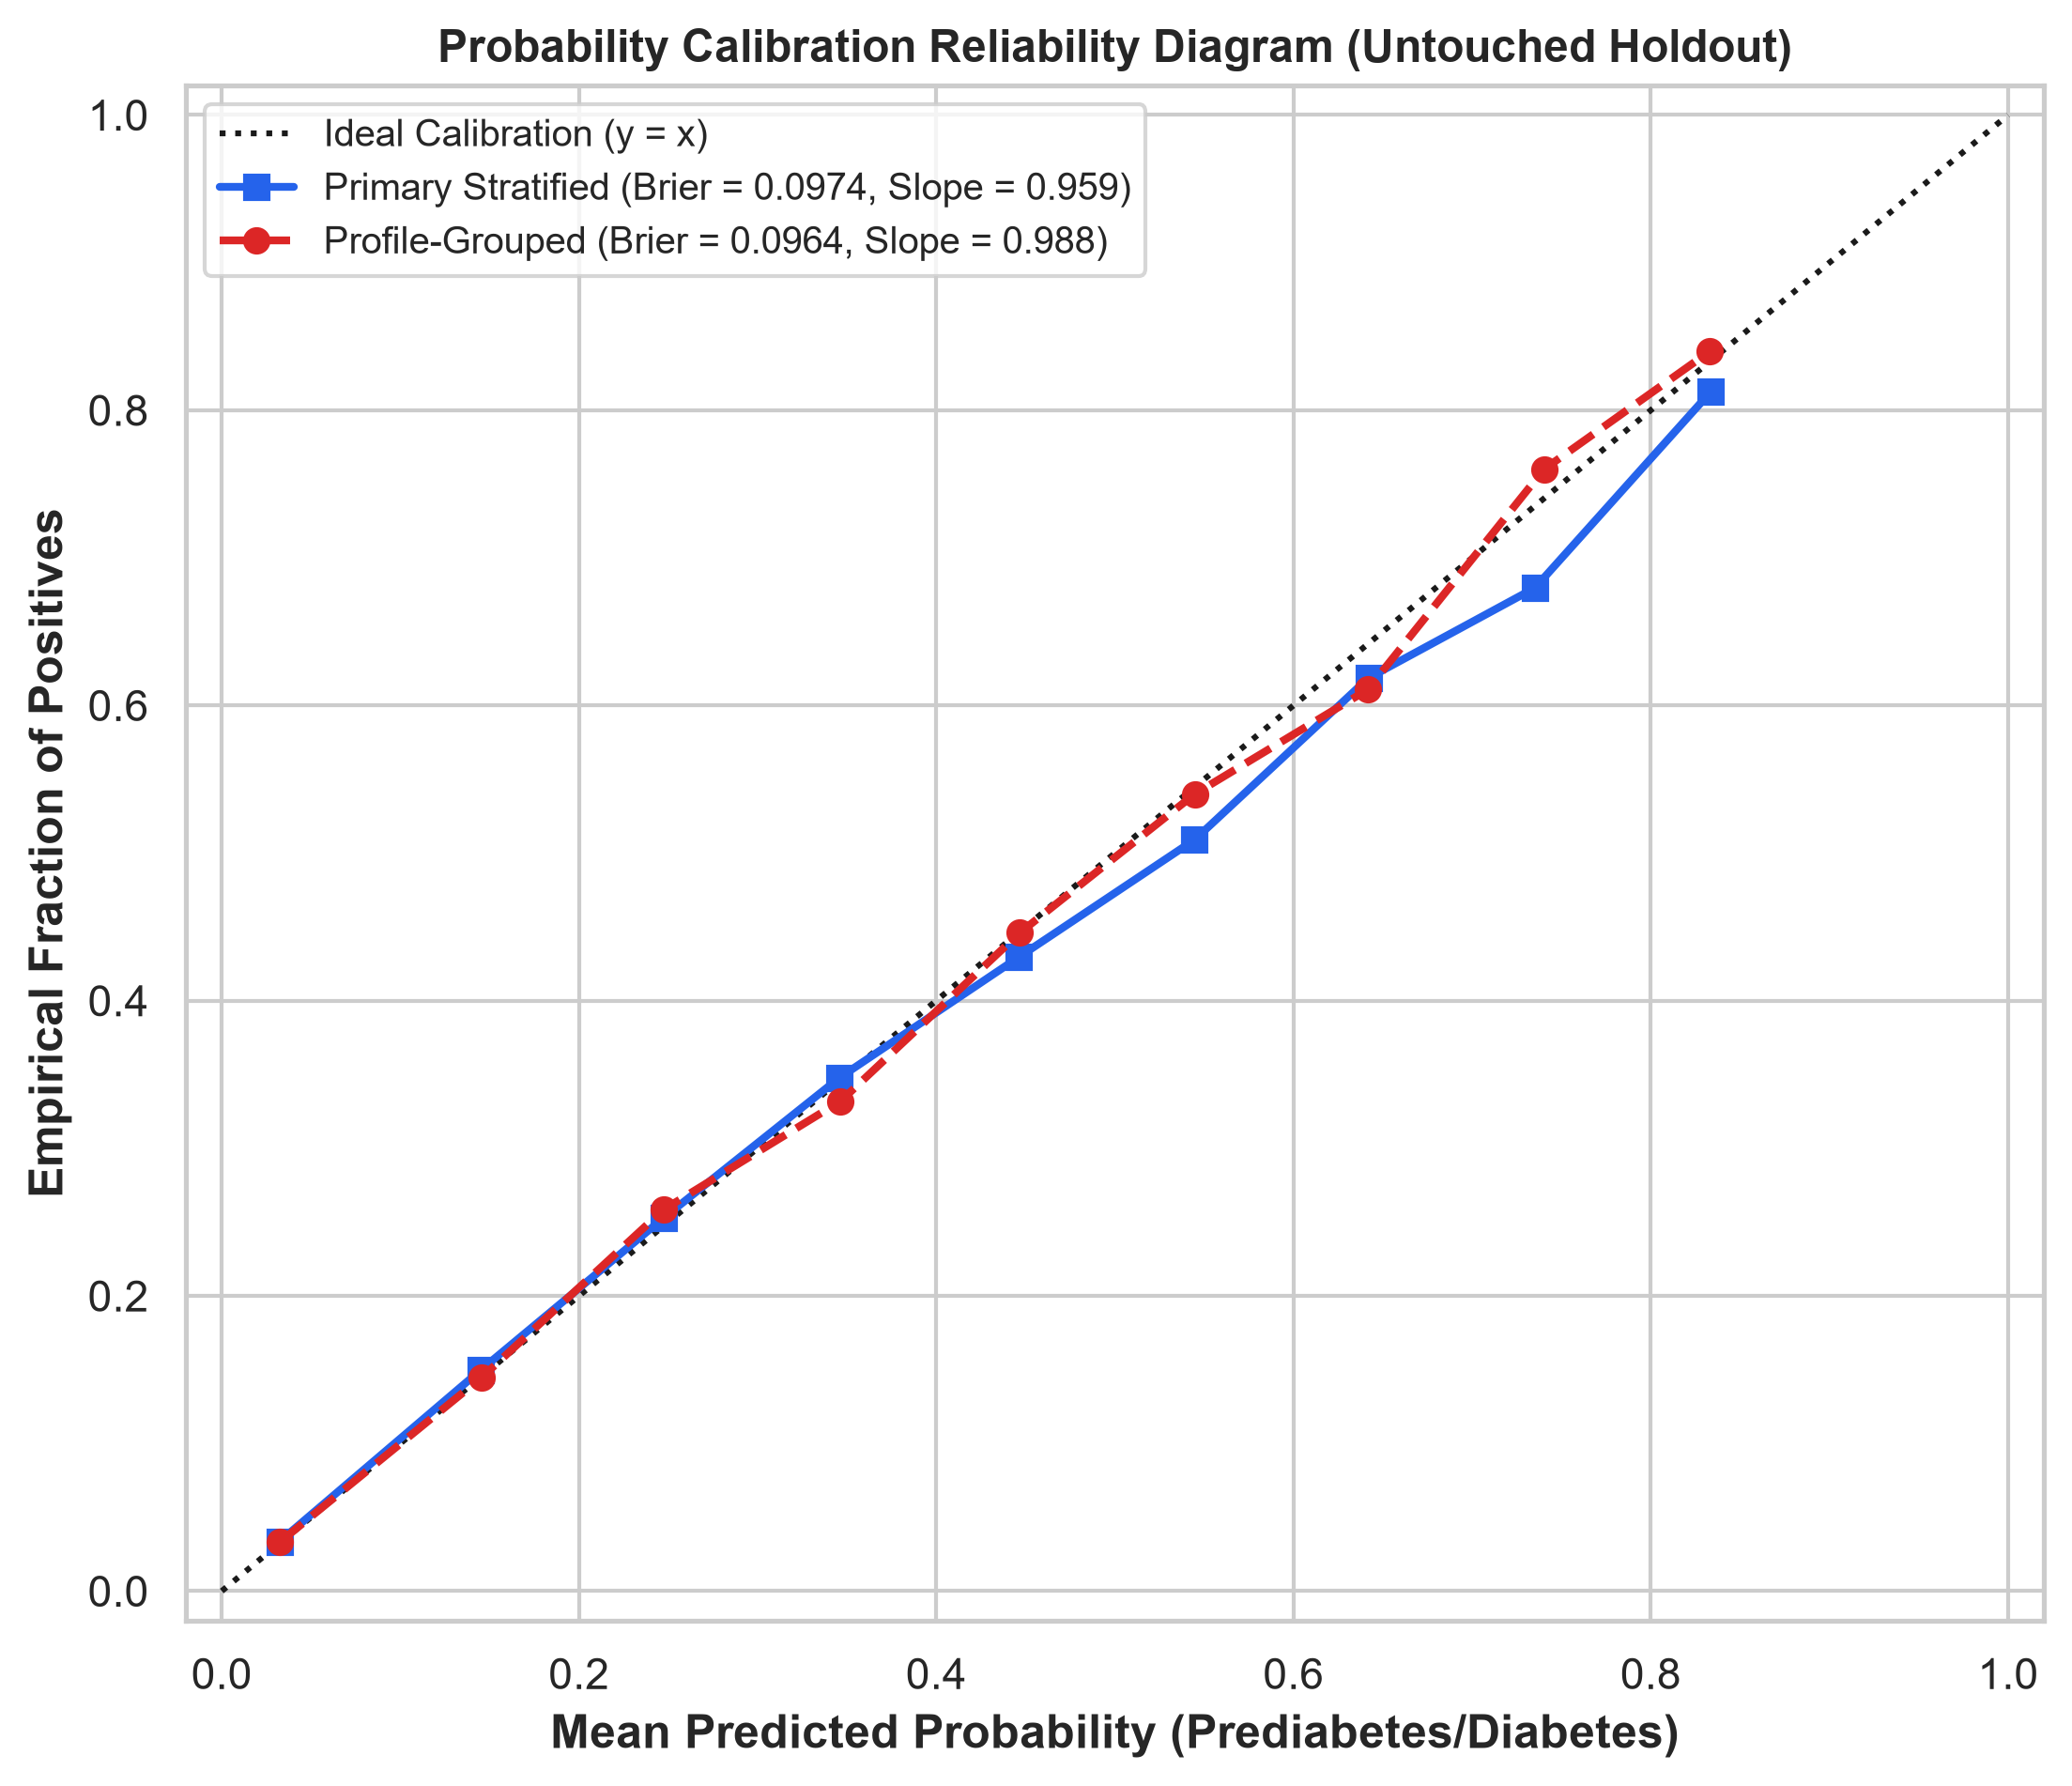
\includegraphics[width=0.85\textwidth]{figure2_calibration_curves.png}
\caption{Calibration curves for the primary stratified evaluation and profile-grouped sensitivity analysis. The grouped evaluation prevents identical predictor profiles from crossing development and holdout partitions.}
\label{fig:calibration_comparison}
\end{figure}

\subsection{SHAP and Statistical Evidence Alignment (RQ3)}
Global SHAP feature attribution identified \texttt{GenHlth} (mean $|\text{SHAP}| = 0.6381$), \texttt{HighBP} (0.5264), \texttt{Age} (0.3994), \texttt{BMI} (0.3978), and \texttt{HighChol} (0.2927) as the five most influential predictors in the XGBoost model. Evidence alignment cross-referencing multivariable likelihood contributions (nested LR $\chi^2$ $\Delta$deviance) categorized all Top-10 features into Group 1 (Consistent High Evidence: \texttt{GenHlth}, \texttt{HighBP}, \texttt{Age}, \texttt{BMI}, \texttt{HighChol}, \texttt{Income}, \texttt{Sex}, \texttt{CholCheck}, \texttt{HeartDiseaseorAttack}, \texttt{HvyAlcoholConsump}), with the remaining 11 secondary features in Group 4 (Table \ref{tab:evidence_alignment}). Because the Top-10 sets under both rankings share 10/10 features in common, all 10 features fall into Group 1 as a direct descriptive consequence of this definition (illustrating complete Top-10 empirical set identity), rather than serving as independent statistical confirmation. 

Because predictors possess differing degrees of freedom after categorical expansion (e.g., \texttt{Age} has 12 degrees of freedom, \texttt{Income} has 7, \texttt{GenHlth} has 4, and binary indicators have 1), we conducted degree-of-freedom-aware sensitivity analyses (Table \ref{tab:rank_sensitivity}). Penalizing feature contributions by parameter dimension ($\text{LR } \chi^2 - \text{df}$) yielded an identical 21-feature ranking and identical concordance with SHAP (Top-10 overlap: 10/10, Jaccard = 1.0000; Spearman $\rho_s = 0.9338$, $p = 6.38 \times 10^{-10}$). Evaluating deviance contribution per parameter ($\text{LR } \chi^2 / \text{df}$) maintained strong alignment (Top-10 overlap: 9/10, Jaccard = 0.8182; Spearman $\rho_s = 0.8818$, $p = 1.27 \times 10^{-7}$), with \texttt{DiffWalk} entering the Top-10 and \texttt{Income} shifting to rank 11. This exploratory internal evidence alignment confirms that the observed concordance is robust to parameter dimensionality.

\begin{table}[htbp]
\centering
\caption{Epidemiological and Machine Learning Evidence Alignment Classification}
\label{tab:evidence_alignment}
\footnotesize
\setlength{\tabcolsep}{2.5pt}
\begin{tabular}{@{}p{3.0cm}p{4.3cm}p{4.5cm}@{}}
\toprule
\textbf{Evidence Group} & \textbf{Features Included} & \textbf{Epidemiological \& Model Interpretation} \\
\midrule
Group 1: Consistent High Evidence (10 features) & \texttt{GenHlth}, \texttt{HighBP}, \texttt{Age}, \texttt{BMI}, \texttt{HighChol}, \texttt{Income}, \texttt{Sex}, \texttt{CholCheck}, \texttt{HeartDiseaseorAttack}, \texttt{HvyAlcoholConsump} & Robust multivariable likelihood contributions (LR $\chi^2$ Top-10) concordant with high gradient-boosted salience (SHAP Top-10); Top-10 set identity is identical across rankings. \\
Group 2: High Statistical, Lower Model Salience (0 features) & None (at Top-10 cutoff) & High multivariable likelihood contribution but secondary tree-based salience. \\
Group 3: High Model Salience, Lower Statistical (0 features) & None (at Top-10 cutoff) & High tree-based salience despite secondary multivariable statistical contribution. \\
Group 4: Consistent Secondary Evidence (11 features) & \texttt{MentHlth}, \texttt{DiffWalk}, \texttt{Education}, \texttt{Stroke}, \texttt{Fruits}, \texttt{PhysHlth}, \texttt{PhysActivity}, \texttt{Smoker}, \texttt{Veggies}, \texttt{AnyHealthcare}, \texttt{NoDocbcCost} & Secondary multivariable contribution and secondary model salience within the analyzed survey sample. \\
\bottomrule
\end{tabular}
\footnotetext{Note: Evidence groups cross-reference feature-level nested Likelihood-Ratio $\chi^2$ ($\Delta$deviance) statistical ranks with Top-10 mean absolute SHAP feature attributions on 10,000 independent holdout observations. Group 1 features represent the descriptive set identity of features appearing in both Top-10 rankings.}
\end{table}

\begin{table}[htbp]
\centering
\caption{Rank Alignment Sensitivity Analysis between SHAP and Statistical Contributions}
\label{tab:rank_sensitivity}
\footnotesize
\setlength{\tabcolsep}{3.5pt}
\begin{tabular}{@{}lccc@{}}
\toprule
\textbf{\shortstack{Rank\\Cutoff}} & \textbf{\shortstack{Primary LR $\chi^2$\\(Overlap / Jaccard)}} & \textbf{\shortstack{df-Aware: LR $\chi^2 - \text{df}$\\(Overlap / Jaccard)}} & \textbf{\shortstack{df-Aware: LR $\chi^2 / \text{df}$\\(Overlap / Jaccard)}} \\
\midrule
Top-5 & 5 / 5 (1.0000) & 5 / 5 (1.0000) & 4 / 5 (0.6667) \\
Top-10 & 10 / 10 (1.0000) & 10 / 10 (1.0000) & 9 / 10 (0.8182) \\
Top-15 & 13 / 15 (0.7647) & 13 / 15 (0.7647) & 13 / 15 (0.7647) \\
\midrule
\multicolumn{4}{l}{\textit{Spearman Rank Correlation Across All 21 Features vs. SHAP:}} \\
\multicolumn{4}{l}{Primary LR $\chi^2$: $\rho_s = 0.9338$ ($p = 6.38 \times 10^{-10}$) \quad $\mid$ \quad LR $\chi^2 - \text{df}$: $\rho_s = 0.9338$ ($p = 6.38 \times 10^{-10}$)} \\
\multicolumn{4}{l}{LR $\chi^2 / \text{df}$: $\rho_s = 0.8818$ ($p = 1.27 \times 10^{-7}$)} \\
\bottomrule
\end{tabular}
\footnotetext{Note: Feature ranking compares XGBoost global mean absolute SHAP importance against multivariable nested Likelihood-Ratio $\chi^2$ ($\Delta$deviance) statistical contributions across all 21 features. Sensitivity analyses account for predictor degrees of freedom ($\text{df}$) using parameter penalization ($\text{LR }\chi^2 - \text{df}$) and average deviance per degree of freedom ($\text{LR }\chi^2 / \text{df}$).}
\end{table}


\section{Discussion}\label{sec:discussion}

\subsection{Screening Utility and Threshold Selection}
The primary empirical finding of this investigation is that conventional machine learning evaluation protocols that rely on default 0.50 decision thresholds are ill-suited for early chronic disease screening. In an imbalanced sample with 13.93\% positive prevalence, a default threshold maximizes overall accuracy (86.52\%) at the expense of clinical utility, failing to detect over 83\% of individuals with prediabetes or diabetes. By optimizing the operational decision threshold to 0.13 on development out-of-fold probabilities, the model attained 80.99\% sensitivity on the untouched holdout partition, decreasing the count of missed positive cases by 77.22\% (from 5,900 to 1,344). Although precision correspondingly decreased to 29.91\%, this represents a favorable operational trade-off for population health screening, where non-invasive initial triage filters individuals for formal diagnostic blood testing.

\subsection{Evaluation Robustness Under Profile Grouping}
A central contribution of this study is the formal evaluation-integrity audit and profile-grouped sensitivity analysis. When survey datasets contain discrete indicators, repeated predictor profiles inevitably emerge. In our sample, 13.47\% of holdout observations share identical predictor profiles with the development set under conventional stratified splitting. To investigate whether this sharing inflated performance or altered model behavior, we conducted a profile-grouped sensitivity analysis enforcing zero profile overlap between partitions.

Re-executing model selection, cross-validation, and threshold selection under grouped partitioning selected XGBoost and the identical screening threshold of 0.13, yielding holdout PR-AUC of 0.4372, ROC-AUC of 0.8310, recall of 81.54\%, precision of 29.93\%, specificity of 69.10\%, Brier score of 0.0964, joint Cox calibration slope of 0.9878, and calibration intercept of $-0.0158$. The close alignment with primary stratified estimates ($\Delta \text{PR-AUC} = +0.0133$, $\Delta \text{Recall} = +0.55\%$, $\Delta \text{Brier} = -0.0010$) provides evidence that the study's primary internal evaluation conclusions are robust to the evaluated partitioning strategy. However, because the primary and profile-grouped holdout sets contain different subsets of survey respondents, this analysis cannot isolate the pure causal effect of profile overlap or definitively prove that overlap has no influence on performance. Rather, the results provide empirical reassurance that the screening utility and calibration behavior observed in this sample are not artifacts of cross-partition profile sharing.

\subsection{Explanatory Grounding and Evidence Alignment}
Explainable AI techniques such as SHAP provide valuable insights into model logic, but unconstrained explanations can mislead if they conflict with established epidemiological evidence. Our evidence alignment framework revealed that all top 10 machine learning predictors demonstrated complete concordance with multivariable statistical likelihood contributions (nested LR $\chi^2$ $\Delta$deviance; Top-10 Jaccard = 1.0000, Spearman $\rho_s = 0.9338$). Discrepancies between unadjusted bivariate associations and multivariable tree attributions were medically interpretable: for example, indicators such as \texttt{DiffWalk} and \texttt{PhysHlth} displayed strong marginal associations but moderate SHAP importance because their predictive variance was largely subsumed by general health rating (\texttt{GenHlth}) and age (\texttt{Age}) in tree splits. Conversely, biological sex demonstrated conditional predictive importance in multivariable boosting despite modest marginal association.

\subsection{Comparison with Literature and Research Contribution}
Rather than claiming unsupported algorithmic novelty or marginal gains in ROC-AUC, this study contributes an integrated methodology for trustworthy survey-based risk prediction across five key dimensions:
\begin{enumerate}
    \item \textbf{Reliability-Oriented Screening Evaluation:} Benchmarking multi-paradigm classifiers prioritized by Precision-Recall AUC under severe class imbalance, avoiding misleading overall accuracy metrics in low-prevalence screening.
    \item \textbf{Development-Only Operating-Point Selection and Calibration Assessment:} Selecting clinical decision thresholds strictly on development out-of-fold probabilities to achieve pre-specified sensitivity ($\ge 80\%$) alongside formal probability calibration diagnostics (Brier scores, Cox calibration slopes and intercepts).
    \item \textbf{Interpretable Statistical--SHAP Evidence Alignment:} Systematically cross-referencing machine learning tree attributions against classical non-parametric and multivariable effect sizes to establish epidemiological grounding and detect potential modeling artifacts.
    \item \textbf{Explicit Data-Integrity Audit of Repeated Profiles:} Disentangling exact full-row duplicate records from identical discrete predictor profiles and conflicting-label observations in anonymized public health surveys.
    \item \textbf{Profile-Grouped Robustness Sensitivity Analysis:} Implementing a controlled sensitivity experiment that enforces zero cross-partition predictor profile sharing through complete grouped redevelopment, empirically evaluating the stability of discrimination, threshold selection, and probability calibration.
\end{enumerate}

\section{Limitations}\label{sec:limitations}

Several limitations must be highlighted:
\begin{enumerate}
    \item \textbf{Cross-Sectional Self-Reported Data:} The BRFSS relies on self-reported survey responses without biochemical confirmation (e.g., fasting plasma glucose, oral glucose tolerance test, or HbA1c). Cross-sectional survey data preclude causal interpretations.
    \item \textbf{Aggregated Target Class:} The target variable combines prediabetes and diagnosed diabetes into a single positive class. While appropriate for broad initial screening, clinical pathways differ substantially between prediabetes management and diabetes pharmacotherapy.
    \item \textbf{Unweighted Sample Analysis:} Our modeling was conducted on the unweighted analyzed sample ($N = 253,680$). Although appropriate for evaluating algorithm behavior, point estimates cannot be directly generalized to US national population prevalence without incorporating complex survey design weights.
    \item \textbf{Internal Validation Only:} Both primary and grouped evaluations are internal splits derived from the 2015 BRFSS wave. While internal holdout evaluation was strictly enforced, transportability to external health systems or different survey years remains unverified.
    \item \textbf{Repeated Predictor Profiles and Identification:} Repeated predictor profiles were present because many BRFSS variables are discrete or ordinal, and respondent identifiers were unavailable. Identical discrete response profiles may legitimately occur among different respondents, and respondent identity cannot be determined from the released analytic dataset. The profile-grouped sensitivity analysis eliminated cross-partition predictor-profile sharing and yielded broadly similar performance estimates. However, this design should be interpreted as a robustness analysis rather than proof that repeated profiles have no effect, because the stratified and profile-grouped holdouts consist of different observations. External and temporal validation remains necessary.
    \item \textbf{Unmeasured Clinical and Biological Variables:} The BRFSS captures self-reported lifestyle and demographic indicators, but omits critical biological predictors such as laboratory biomarkers (fasting blood glucose, oral glucose tolerance, serum lipids, microalbuminuria), genetic risk factors, comprehensive dietary records, and detailed prescription medication histories.
    \item \textbf{Operational Screening Threshold Trade-offs:} Lowering the decision threshold to 0.13 to achieve $\ge 80\%$ sensitivity necessarily increases the false-positive rate, reducing precision to 29.91\%. In practical deployment, this produces approximately 2.3 false-positive screening referrals for every true-positive identified, entailing follow-up clinical evaluation costs that must be managed by the healthcare system.
\end{enumerate}

\section{Future Work}\label{sec:future}

Future research should prioritize:
\begin{itemize}
    \item \textbf{External and Temporal Validation:} Evaluating model transportability on subsequent BRFSS survey waves (e.g., 2017--2023) and external EHR datasets with laboratory biomarkers.
    \item \textbf{Survey-Weighted Machine Learning:} Formulating custom loss functions that incorporate BRFSS complex survey weights to support unbiased population-level risk modeling.
    \item \textbf{Subgroup Fairness and Calibration:} Assessing whether screening thresholds and probability calibration remain equitable across racial, ethnic, age, and socioeconomic subgroups.
    \item \textbf{Multi-Class Risk Stratification:} Developing multi-class models capable of differentiating non-diabetic, prediabetic, and diabetic states.
\end{itemize}

\section{Conclusion}\label{sec:conclusion}

This paper presented an interpretable, screening-oriented machine learning framework for diabetes risk prediction using CDC BRFSS health indicators. By optimizing operational decision thresholds on development out-of-fold probabilities, the selected XGBoost model achieved 80.99\% sensitivity on an independent holdout set, decreasing the count of false negatives by 77.22\% (from 5,900 to 1,344) compared to conventional default cutoffs. Probability calibration assessment yielded sound overall metrics (Brier score 0.0974, slope 0.9589 [95\% CI: 0.9342, 0.9854], intercept $-0.0515$ [95\% CI: $-0.0861$, $-0.0148$]), with the confidence intervals reflecting a modest systematic calibration deviation, and SHAP attributions showed strong concordance with multivariable statistical contributions ($\rho_s = 0.9338$, Top-10 Jaccard = 1.0000). 

A profile-grouped sensitivity analysis further evaluated the stability of the results by preventing identical predictor profiles from crossing development and holdout partitions through complete grouped redevelopment. XGBoost remained the selected model, the development-selected threshold remained 0.13, and discrimination, screening performance, and calibration were broadly consistent with the primary stratified evaluation. These findings support the robustness of the main internal conclusions to partitioning strategy, although they do not replace external or temporal validation. Future population screening initiatives using survey data should routinely adopt screening threshold selection, probability calibration assessment, and evaluation-integrity audits to ensure algorithmic reliability.

\bibliography{references}

\end{document}
